% Drawing 85/05-9 -- folder 85, batch 05, archive page 96 (PDF page 97).
% Transcription: en bas à droite de la feuille, au crayon : un assemblage de tétraèdres autour d'un sommet commun, esquissé et repassé
% Kind: cluster of tetrahedra around a common vertex. Method 2 (schematic redraw from the facsimile). Status: ok.
% Notes: Pencil. Redrawn stroke by stroke on eleven vertices placed once, every stroke between them; heavy strokes where he went over the lines (the upper left triangle, the edges to the common vertex, the lower left triangle and the outline at the right and bottom). Still differs: the sketch is gone over several times and the light strokes (hidden edges, first attempts) are a selection; the solid it shows is not identified. Left out: the faint erased strokes in the middle of the sheet. Redrawn 2026-11-12 (issue 128): to check again. 2026-11-14, Claude Opus 5.5, overlay check (issue 147): rasterised from its own coordinates over the 400 dpi colour scan on a unit grid, corrected and measured (every stroke within 0.7 unit of its pencil on average; all pencil of the sketch within 1.5 units of a stroke except a small doubling at the lower right and specks); not compiled (no TeX in the session). Changed: the light edge from the upper right vertex down to the right vertex moved onto its pencil; added, as drawn on the page, the second stroke along the heavy base of the upper triangle, the short light stroke under its left end and a small dash in the middle of the sketch. The eleven vertices and the heavy and light edges between them lie on the page where they are drawn; which solid it shows is not identified, as before. Status set to ok.
% Coordinates: 1 unit = 1 mm = 1/100 of the crop width (bbox in page fractions: [0.48, 0.6, 0.9, 0.89]).
% Redrawn by Claude (claude-fable-5-2), issue #128, 2026-11-12; not checked by a human; not compiled (no TeX in the session).
% Checked by Claude (claude-opus-5-5) 2026-11-14 (issue #147): overlaid on the 400 dpi colour facsimile, corrected; not compiled (no TeX in the session). Not checked by a human. Status: ok.
% Rights: reproduces part of the work -- behind RENDER_TRANSCRIPTS, never published by itself.
\documentclass[tikz,border=3pt]{standalone}
\usepackage{amsmath,amssymb}
\usetikzlibrary{patterns,arrows.meta}
\tikzset{pencil/.style={black!45}, struck/.style={black!35}, mpt/.style={circle,draw,inner sep=1.3pt}, pt/.style={circle,fill,inner sep=0.9pt}, opt/.style={circle,draw,fill=white,inner sep=1.1pt}}
\begin{document}
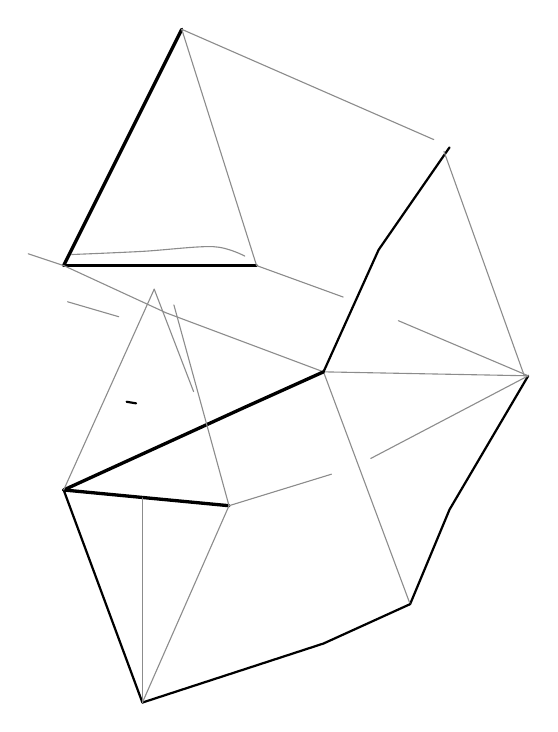
\begin{tikzpicture}[x=1mm,y=1mm,line cap=round,line join=round,font=\scriptsize]
\draw[very thick] (32,-1) -- (17,-31);
\draw[very thick] (17,-31) -- (41.5,-31);
\draw[pencil] (32,-1) -- (41.5,-31);
\draw[pencil] (32,-1) -- (64,-15);
\draw[thick] (66,-16) -- (57,-29) -- (50,-44.5);
\draw[pencil] (65.3,-16.5) -- (75.5,-45);
\draw[pencil] plot[smooth, tension=0.55] coordinates {(18,-29.6) (27,-29.2) (36,-28.6) (40,-29.8)};
\draw[pencil] (17.5,-35.6) -- (24,-37.5);
\draw[thick] (25,-48.3) -- (26.2,-48.5);
\draw[pencil] (50,-44.5) -- (76,-45);
\draw[thick] (76,-45) -- (66,-62) -- (61,-74);
\draw[pencil] (50,-44.5) -- (61,-74);
\draw[pencil] (12.5,-29.5) -- (17,-31) -- (30,-37) -- (50,-44.5);
\draw[very thick] (17,-59.5) -- (40,-49) -- (50,-44.5);
\draw[very thick] (17,-59.5) -- (38,-61.5);
\draw[pencil] (38,-61.5) -- (51,-57.5);
\draw[thick] (17,-59.5) -- (27,-86.5);
\draw[thick] (27,-86.5) -- (50,-79) -- (61,-74);
\draw[pencil] (28.5,-34) -- (17,-59.5);
\draw[pencil] (28.5,-34) -- (33.5,-47);
\draw[pencil] (31,-36) -- (38,-61.5);
\draw[pencil] (27,-86.5) -- (38,-61.5);
\draw[pencil] (27,-86.5) -- (27,-60.5);
\draw[pencil] (41.5,-31) -- (52.5,-35);
\draw[pencil] (59.5,-38) -- (76,-45);
\draw[pencil] (76,-45) -- (56,-55.5);
\end{tikzpicture}
\end{document}
